%\newpage

% ****************************************************************************************
\chapter{Einführung}
\label{chap:Einfuehrung}
% ****************************************************************************************



%\pagebreak

% ****************************************************************************************
\section{Problemformulierung}
\label{sec:Problemformulierung}
% ****************************************************************************************
Die vorliegende Arbeit beschäftigt sich mit dem Design, der Simulation sowie der Implementierung eines digitalen Echtzeitsystems zur Lokalisierung einer bewegten Sprachquelle innerhalb eines geschlossenen Raumes. Ziel ist die Erstellung eines Algorithmus, der auf Basis geeigneter Schätzverfahren die Richtung (Horizontal- und Vertikalwinkel) dieser Signalquelle, bezogen auf ein Referenzkoordinatensystem, ermittelt (\abb{Sprecher_In_Raum}). Als zugrunde liegendem theoretischen Ansatz zur Bestimmung der Schalleinfallsrichtung (DOA\footnote{Direction-Of-Arrival}) eines Quellensignals werden hier die Laufzeitunterschiede (TDOA\footnote{Time-Difference-Of-Arrival}) zwischen den einzelnen Mikrofonen sowie die bekannte Geometrie der Mikrofonanordnung\footnote{Mikrofonarray} ausgenutzt. Eine graphische Darstellung soll letztlich mittels serieller Übertragung der geschätzten Ergebnisse an ein Anzeigegerät realisiert werden.

% ------------------------------------------ FIGURE --------------------------------------
\myFigure{real}
         {big}
         {htbp}
         {Richtungsbestimmung einer bewegten Sprachquelle im Raum.}
         {Sprecher_In_Raum} 
         {01_Einfuehrung/Sprecher_In_Raum}
% ------------------------------------------ FIGURE --------------------------------------

Zur Lösung diese Aufgabenstellung stehen ein kugelförmiges Mikrofonarray mit acht Kondensatormikrofonen (\abb{Foto_MikrofonArray}) inkl. Mikrofonvorverstärker, ein leistungsstarker digitaler Signalprozessor (\abb{Foto_DSP}) der Firma \ti sowie ein Desktopcomputer zur Verfügung.

% ----------------------------------------- SUB-FIGURE -----------------------------------
\begin{figure}
        \centering
        \begin{subfigure}[b]{0.435\textwidth}
                \centering
                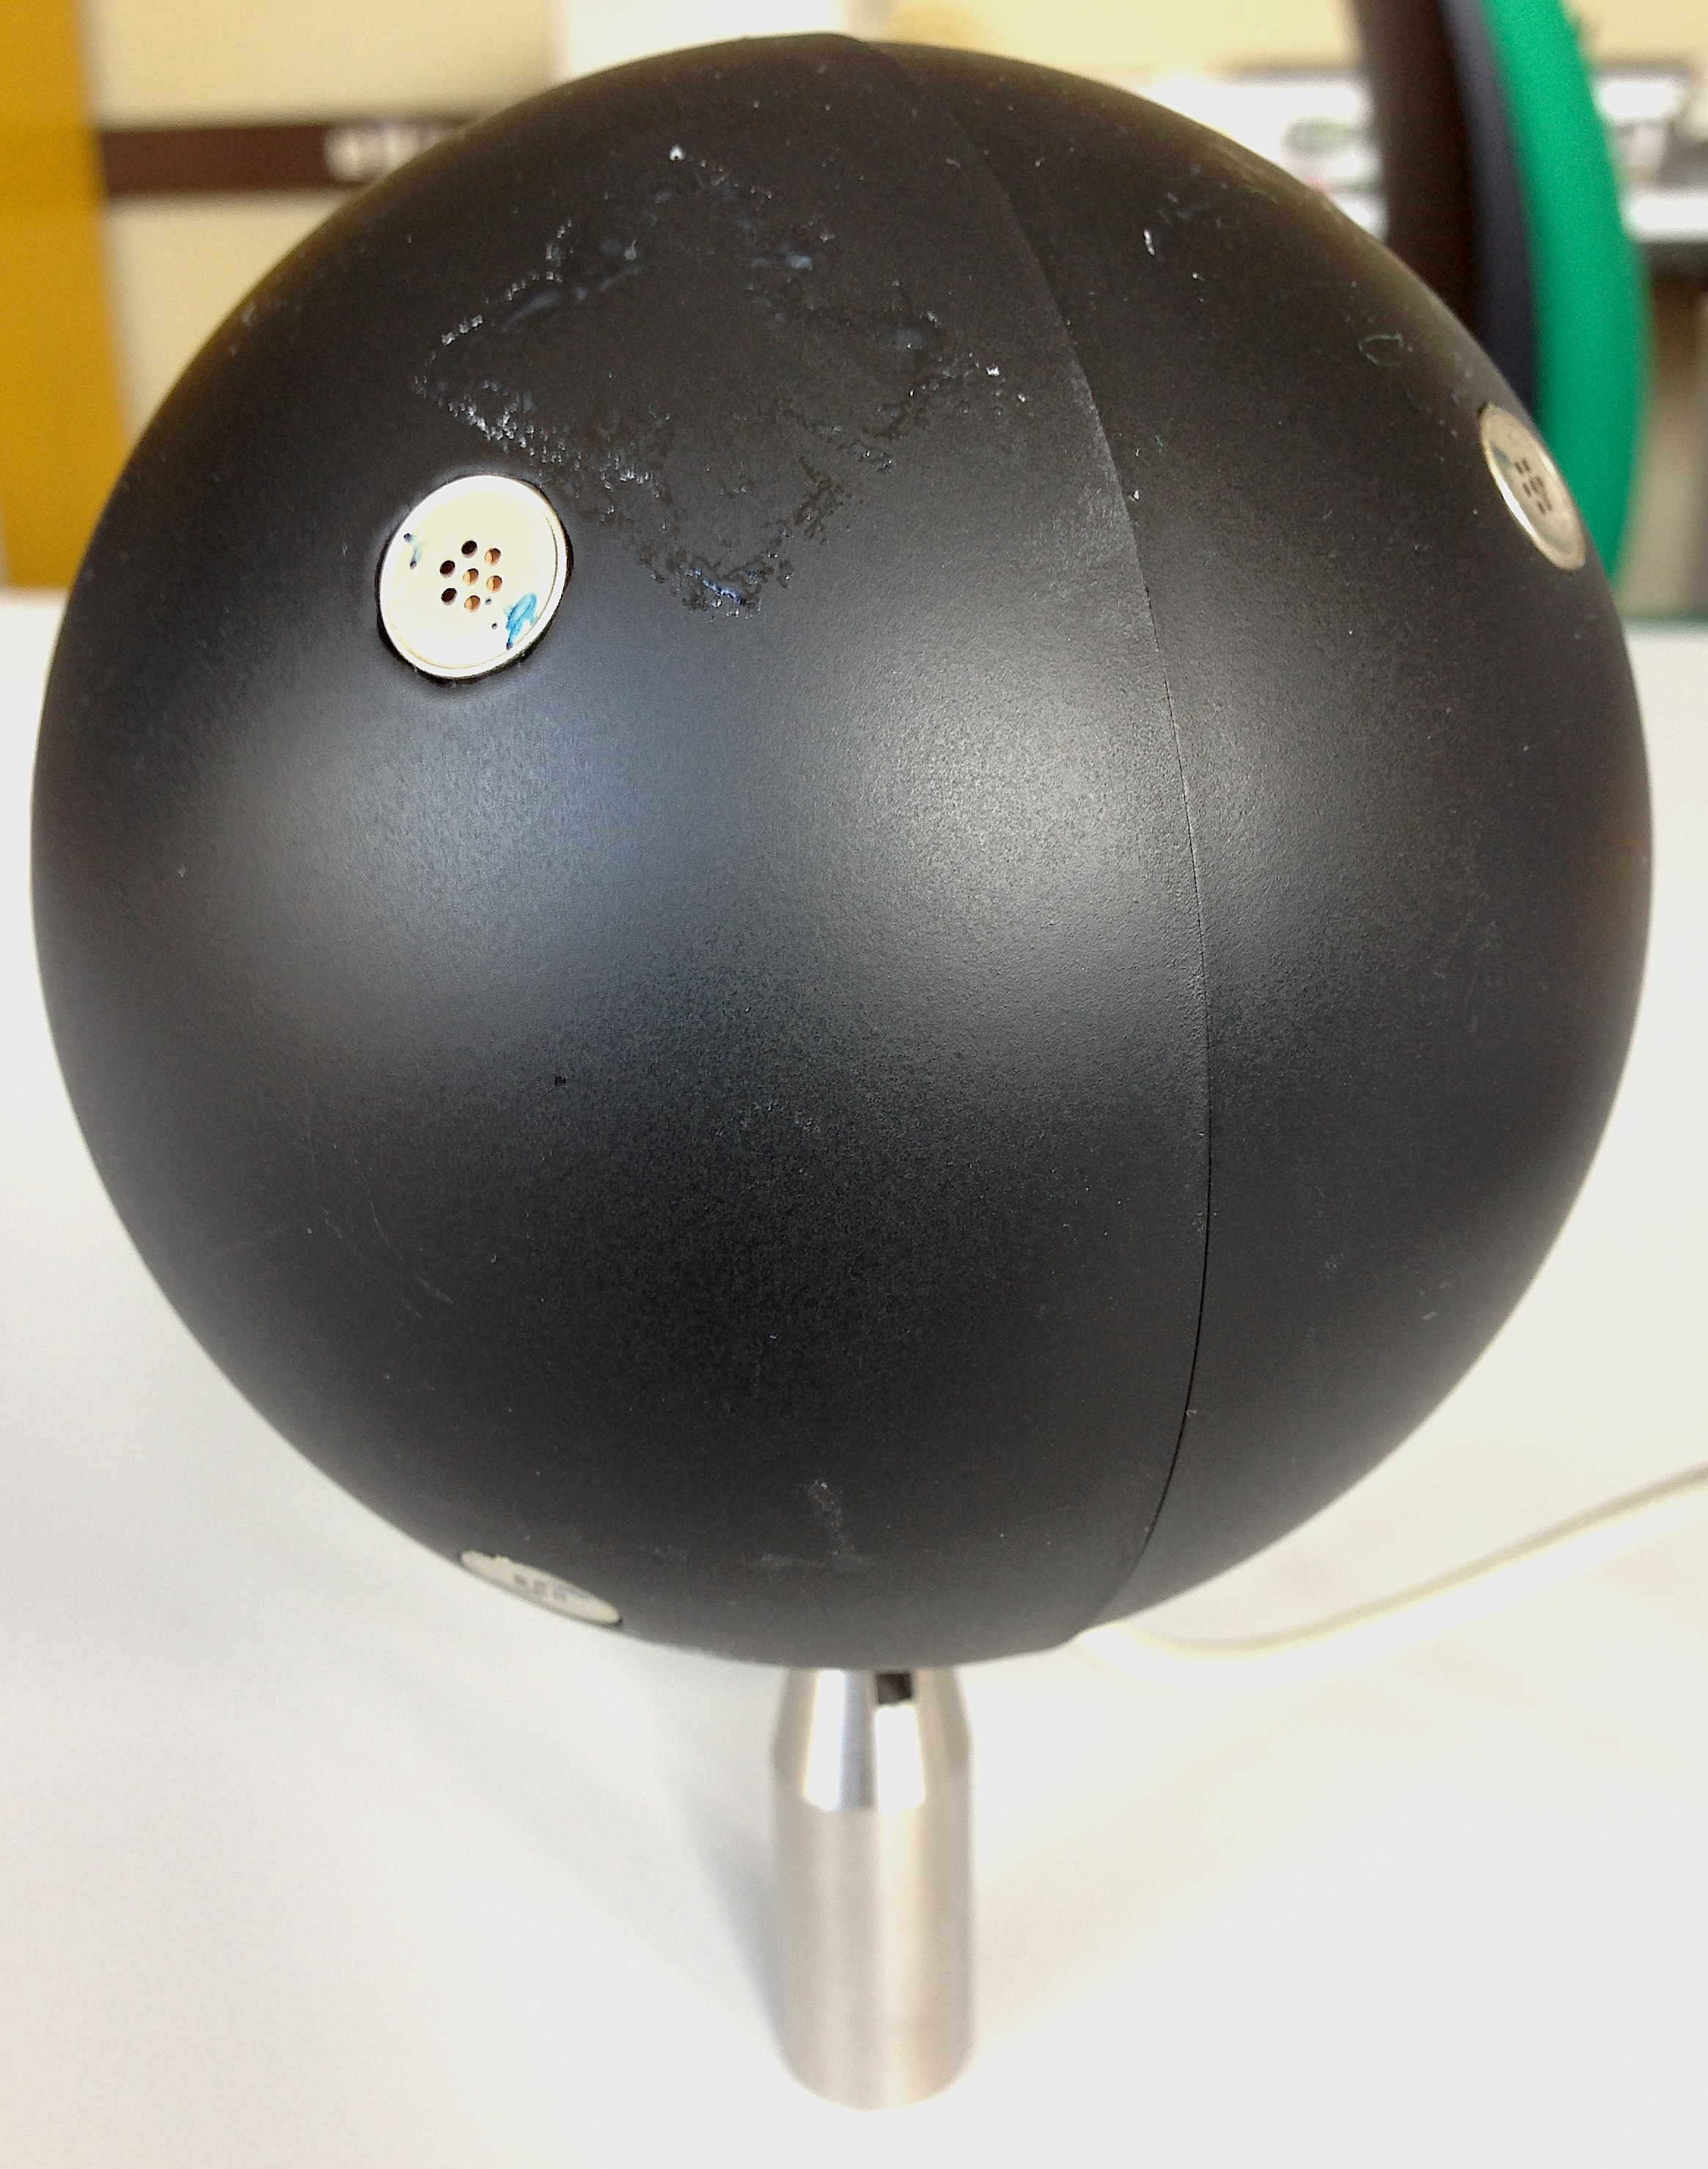
\includegraphics[width=\textwidth]{grafiken/01_Einfuehrung/Foto_MikrofonArray}
                \caption{kugelförmiges Mikrofonarray}
                \label{fig:Foto_MikrofonArray}
        \end{subfigure}
        ~ %add desired spacing between images, e. g. ~, \quad, \qquad etc.
          %(or a blank line to force the subfigure onto a new line)
        \begin{subfigure}[b]{0.48\textwidth}
                \centering
                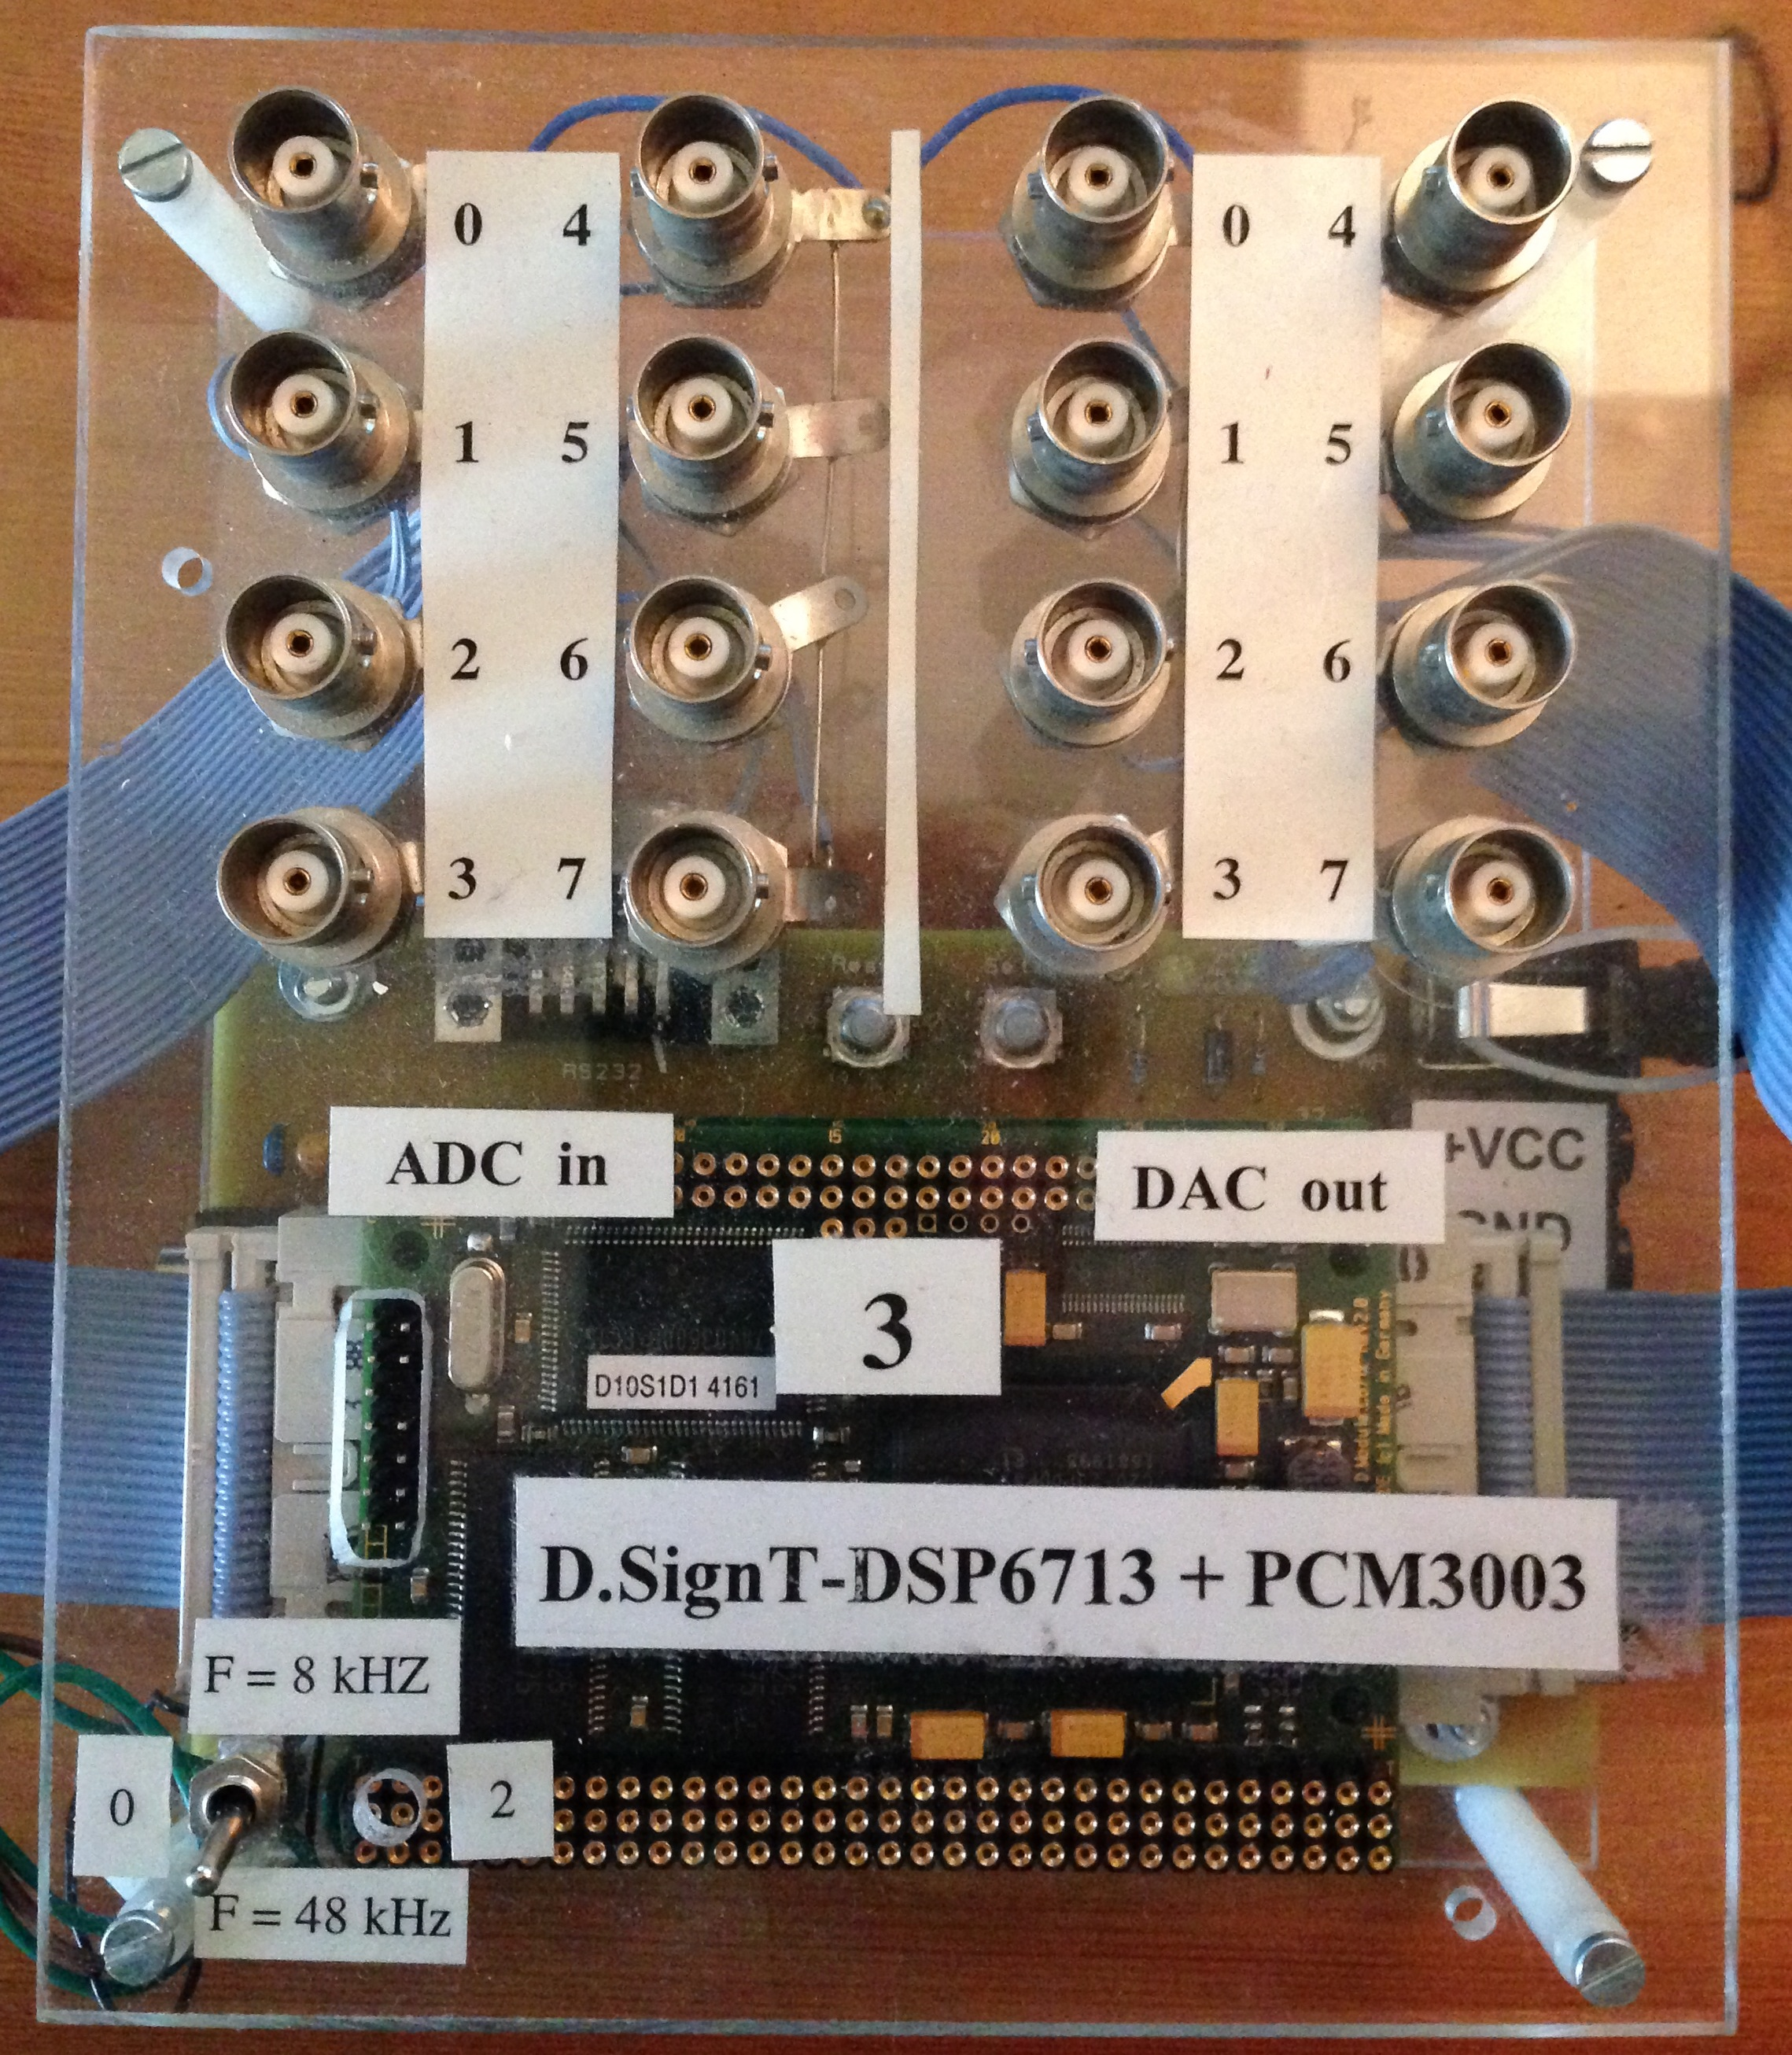
\includegraphics[width=\textwidth]{grafiken/01_Einfuehrung/Foto_DSP}
                \caption{Digitaler Signalprozessor}
                \label{fig:Foto_DSP}
        \end{subfigure}
        \caption{Verwendete Hardware}
        %\caption{Verwendete Hardware}
\end{figure}
% ----------------------------------------- SUB-FIGURE -----------------------------------



\abb{Blockschaltbild_System} zeigt ein Prinzip-Blockschaltbild des Systems. Dieses lässt sich wie dargestellt in einen analogen -und digitalen Systemabschnitt klassifizieren. Im Rahmen dieser Arbeit soll die Signalverarbeitung im digitalen Systemabschnitt im Vordergrund stehen, da bereits alle Komponenten des Analogabschnitts funktionsfähig zur Verfügung gestellt wurden.

Die Ergebnisse dieser Arbeit wurden auf Basis von \citet{Master_Array_Pikora}, \citet{Master_Array_Mueller} sowie des in \citet[S. 196ff]{Book_Array_Benesty} und \citet{Paper_Array_Benesty} beschriebenen Verfahrens des Mehrkanal-Kreuzkorrelationskoeffizienten (MCCC\footnote{Multichannel Cross-Correlation Coeffcient}) erzielt.


% ------------------------------------------ FIGURE --------------------------------------
\myFigure{real}
         {max}
         {htbp}
         {Blockschaltbild des Detektionssystems}
         {Blockschaltbild_System} 
         {01_Einfuehrung/Blockschaltbild_System}                                
% ------------------------------------------ FIGURE --------------------------------------

% Die Richtungsinformation der Quelle kann so unter Berücksichtigung der geometrische Zusammenhänge zwischen Schallwelle und Mikrofonarray aus der Laufzeitdifferenz zwischen den Mikrofonen extrahiert sowie auf ein beliebiges Koordinatensystem abgebildet werden.



% Hier noch was zum Koordinatensystem, den beiden Winkeln und absolute position des Arrays, fernfeld usw. schreiben.


% ****************************************************************************************
\section{Zielsetzung}
\label{sec:Zielsetzung}
% ****************************************************************************************
Auf Basis der unter \Sec{sec:Problemformulierung} genannten Problemstellung lassen sich folgende vom System zu erfüllende Ziele definieren:

\begin{enumerate}
    \item Fähigkeit zur Verarbeitung breitbandiger Signale wie Sprache
    \item Fähigkeit zur räumlichen Richtungsdetektion der Quelle mit ausreichend hoher Genauigkeit (Horizontal- sowie Vertikalwinkel)
    \item Fähigkeit zum Einsatz in Umgebungen mit hohem Rauschanteil und/oder Reflexionsfaktor
    \item Fähigkeit zur Datenverarbeitung in Echtzeit
\end{enumerate}

Der Begriff "`Echtzeit"' lässt sich dabei wie folgt definieren: \\

\definition{Ein Programm rechnet in Echtzeit, wenn es Eingabedaten so schnell verarbeitet, wie der Vorgang, der sie erzeugt. \cite[S. 34]{Slide_ImageProcess_Koelzer}}


Im Hinblick auf eine spätere Implementierung mit Verwendung eines digitalen Signalprozessors lassen sich aus den oben genannten Zielen folgende Forderungen spezifizieren, um eine ordnungsgemäße Funktion des Gesamtsystems zu gewährleisten:

\begin{enumerate}
    \item Verarbeitung von Sprachsignalen bis zu einer oberen Grenzfrequenz von $f_{max} = 3 kHz$
    \item Robustes Verfolgen einer Sprachquelle innerhalb eines definierten Winkelraums:
        \begin{itemize}[label = \textbullet]
            \item Azimuth: $0° \leq \theta < 360°$
            \item Elevation: $-90° < \phi < 90°$
        \end{itemize}
    \item Die Dauer der Datenverarbeitung muss gleich oder kleiner der Datenaufzeichnungsdauer sein. Demzufolge muss die Bedingung $T_{Processing} \leq T_{Frame}$ dauerhaft erfüllt sein.
    \item Der Prozess von Datensammlung und Datenverarbeitung muss zwingend nebenläufig stattfinden.
    \item Zur Sicherstellung der Ergebniskontinuität muss ein kontinuierlicher Datenstrom zwischen Ein- und Ausgabeschnittstelle gewährleistet sein. 
\end{enumerate}

